\documentclass[
	article,
	12pt,
	openright,
	twoside,
	a4paper,
	english,
	brazil % Idioma principal
]{abntex2}

\usepackage[brazil]{babel}
\usepackage[utf8]{inputenc} % Caracteres acentuados. utf8 é comum no linux
\usepackage[T1]{fontenc}
\usepackage{lmodern} % Usa fontes modernas e evita substituições de fontes
\usepackage{multirow}
\usepackage{float}
\usepackage{mathtools}
\usepackage{amsmath}
\usepackage[top=3cm,bottom=2cm,left=3cm,right=2cm]{geometry}
\usepackage{appendix}
\usepackage{hyperref}
\usepackage{amssymb}
\usepackage{subfig}
\usepackage{upgreek}
\usepackage[alf, abnt-etal-list=0]{abntex2cite}	% Citações padrão ABNT
\usepackage{graphicx} % Inclusão de figuras
\usepackage{color}
\newcommand{\hilight}[1]{\colorbox{cyan}{#1}}
\usepackage{pdfpages}

\graphicspath{ {./charts} }

\urlstyle{same}

\hypersetup{
	pdfauthor={-},
	pdftitle={Projeto IC},
	colorlinks=true,
	linkcolor=black,
	citecolor=black,
	urlcolor=black,
	bookmarksopen=true,
	pdfstartview={FitH},
	plainpages=false, % Coloca links no pdf
}

\DoubleSpacing\makeindex

\begin{document}
	\selectlanguage{brazil}
	\pagestyle{empty}
	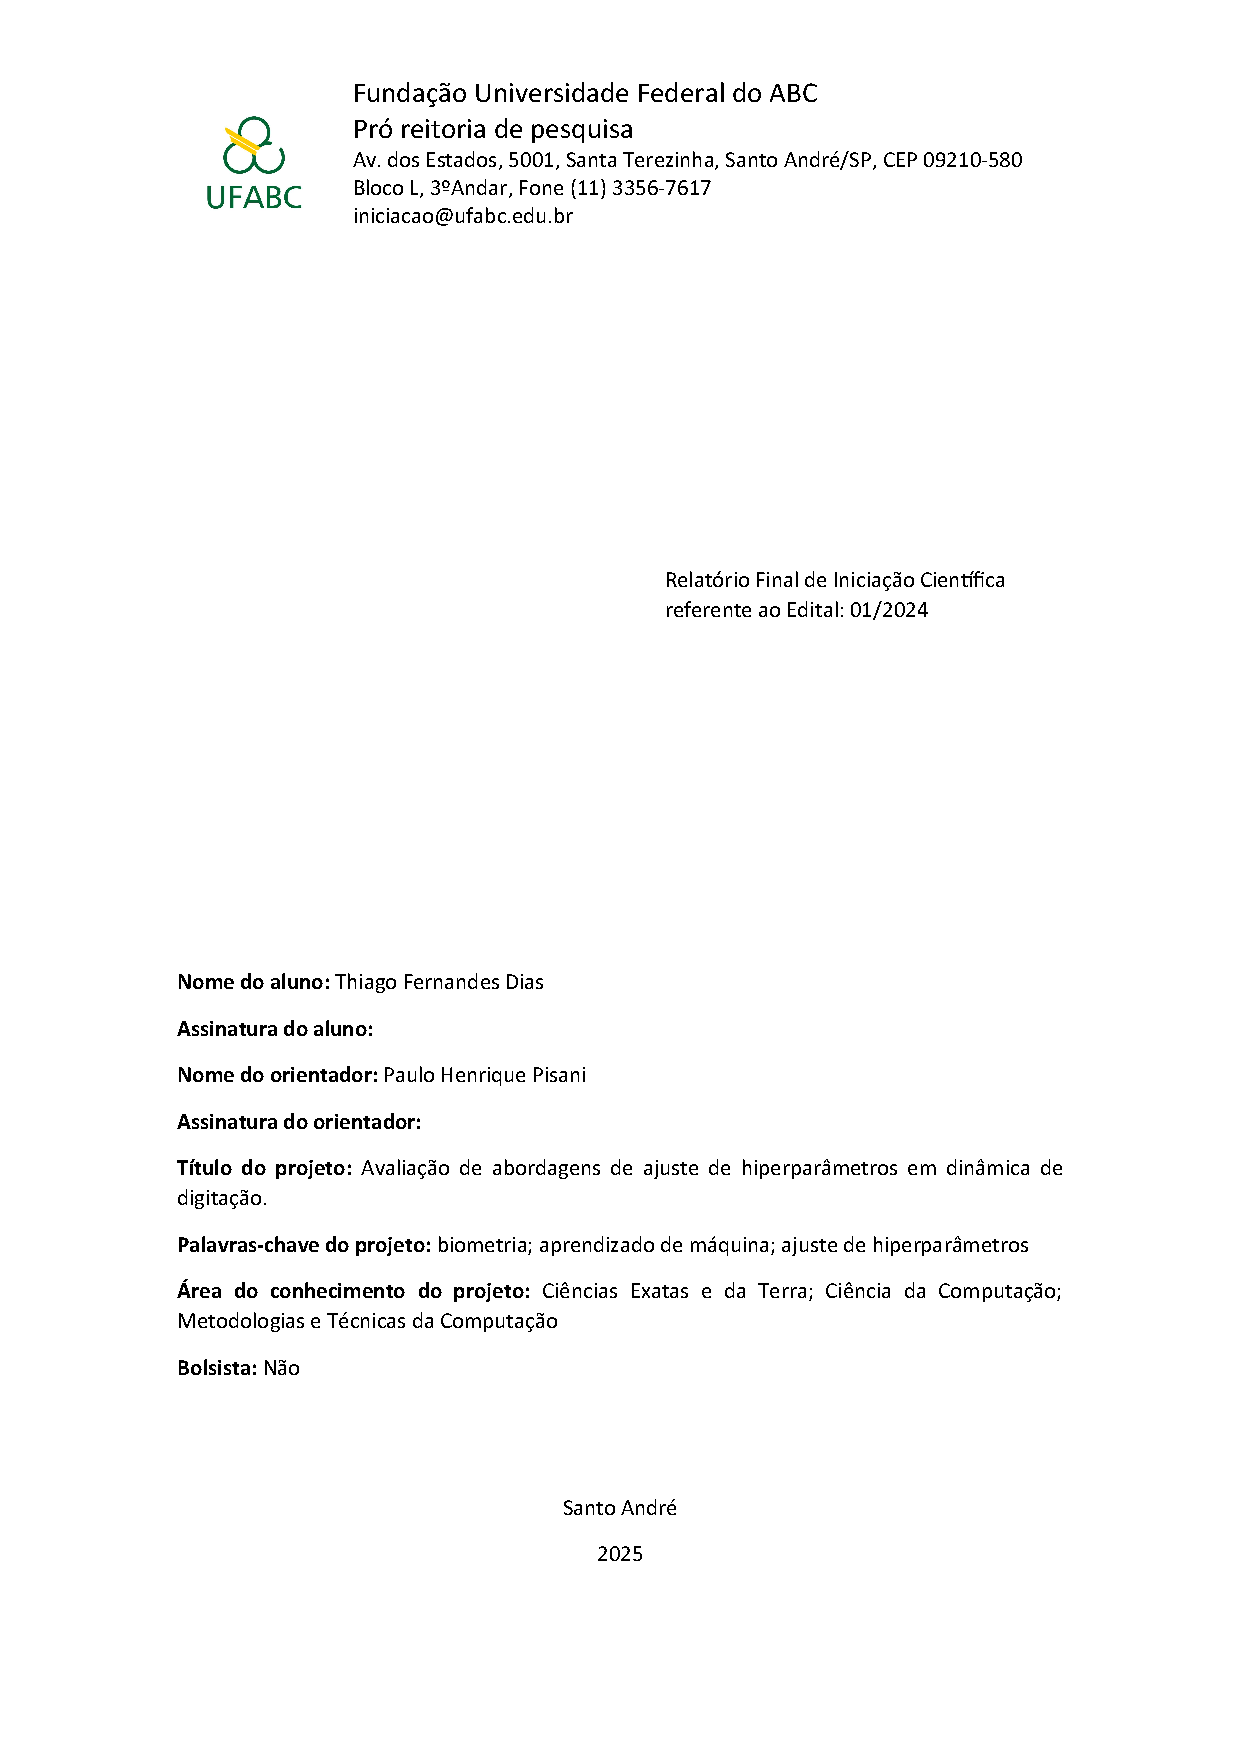
\includepdf[pages={1}]{capa_projeto.pdf}
	\section*{Resumo}

O uso de biometria para autenticação de usuários, em oposição a métodos tradicionais baseados em senhas estáticas, têm sido atrativo em razão da maior segurança que um sistema biométrico pode proporcionar. Os usuários podem ser reconhecidos com base em características físicas ou comportamentais ao invés de precisarem se lembrar de uma senha ou a ter em mãos um cartão inteligente ou \textit{token}. Dentre as diversas modalidades biométricas existentes, há a \textit{dinâmica de digitação}, que reconhece as pessoas com base em seu ritmo de digitação. Diversos algoritmos de classificação podem ser usados nesse contexto. Esses algoritmos possuem hiperparâmetros, que precisam ser ajustados adequadamente. O ajuste de hiperparâmetros pode ser realizado para cada usuário individualmente ou pode ser global, isso é, os hiperparâmetros assumirão o mesmo valor para todos os usuários. O objetivo deste projeto é explorar diferentes abordagens de ajuste de hiperparâmetros em algoritmos para classificação para dinâmica de digitação.
	\tableofcontents*
    \clearpage
    \section{Introdução}\label{sec:introduacao}

Nos últimos anos, a popularização de serviços oferecidos única e exclusivamente pela da Internet tem crescido de forma extraordinária. Muitas pessoas realizam pagamentos em sites de lojas diretamente de suas casas e gerenciam suas contas bancárias sem a necessidade de irem até os bancos~\cite{seguranca_de_dados}. Dessa forma, surge a necessidade sistemas de autenticação e identificação cada vez mais sofisticados.

Entretanto, na perspectiva de~\citeonline{Ryu2023Design}, a maioria dos sistemas de autenticação comumente usados são baseados em senhas estáticas, ou uma combinação entre uma senha e um cartão inteligente ou~\textit{tokens}.~\citeonline{Peacock2004} destacam que essa abordagem possui uma série de limitações. Por exemplo, senhas compostas por palavras comuns, sequências numéricas ou alfanuméricas simples que sejam passíveis de memorização são consideradas ``fracas'' no que se refere ao nível de segurança que elas oferecem, pois podem ser descobertas por ataques do tipo ``força bruta''.

~\citeonline{Peacock2004} ainda afirmam que é recomendado que os usuários criem senhas maiores e compostas por uma combinação de números, letras e caracteres especiais para serem menos vulneráveis a ataques. Em adição a isso, as senhas deveriam ser diferentes para cada conta nos sites em que acessam. Todavia, muitas vezes os usuários ainda optam pela utilização de uma mesma senha para todas as suas contas, o que gera um risco de segurança: se apenas um dos sistemas for invadido e tiver os seus dados roubados, o acesso aos dados do indivíduo em todos os outros serviços estará comprometido.

Segundo~\citeonline{biometrics_a_tool_for_information_security}, muitas dessas limitações associadas ao uso de senhas podem ser contornadas pela incorporação de métodos de autenticação melhores. Nesse sentido, a biometria, como uma forma de estabelecer a identidade por meio de características físicas ou comportamentais dos indivíduos, surge como uma alternativa. Há diversas modalidades biométricas~\cite{Jain2016_50Years}.

Neste projeto, será dado o enfoque na vertente comportamental, em particular, na~\textit{dinâmica de digitação}~\cite{Roy2022systematic}. Essa modalidade biométrica envolve analisar a forma com que um indivíduo digita em um teclado~\cite{monrose2000keystroke}. Os usuários são então reconhecidos com base no seu ritmo de digitação.

Conforme definido em~\cite{Jain2004_IntroToBiometrics}, sistemas biométricos são sistemas de reconhecimento de padrões que extraem características de dados biométricos e então comparam as características extraídas com uma referência biométrica em um banco de dados~\cite{Jain2004_IntroToBiometrics}. Essa comparação das características extraídas a partir dos dados biométricos com a referência biométrica no banco de dados frequentemente resulta em uma pontuação (\textit{score})~\cite{Jain2016_50Years}. Assumindo que seja uma pontuação indicando a similaridade, a classificação pode ser realizada aplicando um limiar de corte (\textit{threshold}). Se a pontuação for maior que o limiar, o dado biométrico é classificado como genuíno e, caso contrário, como sendo de um impostor.

Nesse contexto, o limiar de corte pode ser entendido com um hiperparâmetro. O trabalho de~\cite{hpo_foundations_algorithms_and_open_challenges} menciona o limiar de corte como um hiperparâmetro em algoritmos que retornam uma pontuação ou uma probabilidade. Outros algoritmos usados para reconhecimento de usuários pela dinâmica da digitação podem possuir outros hiperparâmetros para serem ajustados. Os valores dos hiperparâmetros tem impacto importante no desempenho preditivo de um sistema biométrico.

O objetivo deste projeto é comparar diferentes abordagens para ajuste de hiperparâmetros em algoritmos de classificação para dinâmica de digitação. Sobre esse aspecto, há algumas questões que podem ser investigadas. A primeira é sobre realizar o ajuste de forma global ou individualizada para cada usuário no sistema biométrico. Em biometria, o limiar de corte pode ser um valor global comum para todos os usuários ou um valor específico para cada usuário~\cite{Giot2011Unconstrained, Mhenni2019DoubleSerial}. Esse conceito pode ser estendido para outros hiperparâmetros, determinando os valores de forma comum a todos os usuários ou de forma individualizada. Outra questão que pode ser estudada neste contexto é sobre a técnica de ajuste de hiperparâmetros.

As demais seções do projeto estão organizadas da seguinte forma: na Seção~\ref{sec:fundamentacao_teorica}, são introduzidos conceitos sobre dinâmica da digitação e ajuste de hiperparâmetros; na Seção~\ref{sec:metodologia} são descritos os conjuntos de dados utilizados e suas particularidades e os experimentos realizados; na Seção~\ref{sec:resultados} são expostos os resultados e é feita uma discussão sobre eles e; na Seção~\ref{sec:conclusao} é feita a conclusão do projeto


\section{Fundamentação Teórica}\label{sec:fundamentacao_teorica}

Esta seção apresenta alguns conceitos importantes para este projeto de pesquisa envolvendo dinâmica da digitação e ajuste de hiperparâmetros.


\subsection{Dinâmica da digitação}\label{subsec:dinamica_de_digitacao}

A dinâmica da digitação é um modalidade biométrica comportamental que diferencia os indivíduos com base em atributos característicos da digitação de textos, como o tempo em que o indivíduo permanece pressionando cada tecla, o intervalo de tempo entre cada ativação de tecla e padrões nos erros de digitação~\cite{biometric_personal_auth_using_keystroke_dynamics}.

Segundo~\citeonline{Peacock2004}, a principal vantagem da dinâmica da digitação em relação às demais modalidades biométricas comportamentais é a sua transparência. Por exemplo, se usada em conjunto com um formulário de autenticação comum, composto por um identificador de usuário (ou nome de usuário,~\textit{username}) e uma senha, as métricas de digitação podem ser obtidas das informações que o indivíduo necessariamente deverá inserir no sistema que ele deseja acessar. Além disso, em serviços baseados na Web, muitas vezes não é viável exigir formas de autenticação por biometria, pois os usuários podem não ter acesso aos dispositivos necessários, como câmeras e sensores de impressões digitais, ou equipamentos mais sofisticados.

Para fins de reconhecimento biométrico, os dados podem ser obtidos por meio dos padrões de digitação tanto de~\textit{textos fixos} definidos previamente, que os usuários serão requisitados a digitar para fins de identificação ou verificação, ou de~\textit{textos livres}, sem um tamanho fixo ou qualquer outra restrição. Muitos dos estudos desenvolvidos sobre autenticação pela dinâmica de digitação consideram um mecanismo baseado em texto fixo, geralmente o nome de usuário e a senha coletados previamente. Entretanto, diversos pesquisadores também aplicam algoritmos de aprendizado de máquina para desenvolver modelos capazes de autenticar os usuários de forma contínua por meio do texto digitado em um sistema durante o seu uso~\cite{continuous_auth_by_free_text_keystroke_based_on_cnn_and_rnn}.


\subsubsection{Coleta e modelagem de dados}\label{subsubsec:coleta_e_modelagem}

Considerando uma situação em que o texto a ser digitado é fixo, para criar modelos de Aprendizado de Máquina capazes de realizar a verificação de usuários a partir da forma com que eles digitam o texto pré-determinado é necessário um processo de treinamento a partir dos dados coletados durante a digitação do texto. Além disso, esses dados devem ser modelados corretamente para que sejam utilizados nos algoritmos de Aprendizado de Máquina.

Enquanto o usuário digita o texto são registrados os intervalos de tempo de ativação entre as teclas, sendo eles~\cite{Dias2023keyrecs}:

\begin{itemize}
    \item{\textit{Hold time}, ou~\textit{Dwell time}}: tempo em que o usuário permaneceu pressionando uma tecla após a ativação;
    \item{\textit{Down-Down}, ou~\textit{Flight time}}: intervalo de tempo entre a ativação de duas teclas consecutivas;
    \item{\textit{Down-Up}}: intervalo de tempo entre a ativação de uma tecla e a desativação da próxima tecla
    \item{\textit{Up-Down}}: intervalo de tempo entre a desativação de uma tecla e ativação da próxima tecla;
    \item{\textit{Up-Up}}: intervalo de tempo entre a desativação de duas teclas.
\end{itemize}

A cada vez que um participante digita o texto fixo, esses intervalos são registrados. Eles compõem um vetor, que serve como dado de entrada em algoritmos de Aprendizado de Máquina. 


\subsection{Hiperparâmetros}\label{subsec:ajuste_de_hiperparametros}

De acordo com~\citeonline{on_hyperparameter_optimization_of_machine_learning_algorithms}, desenvolver um modelo de aprendizado de máquina que seja efetivo na resolução de um determinado problema é uma tarefa complexa e demorada. Ela envolve a escolha do algoritmo apropriado e a obtenção de um modelo arquitetural ótimo por meio do ajuste de hiperparâmetros. O autor explica que há dois tipos de parâmetros em modelos de aprendizado de máquina: os~\textit{parâmetros} do próprio modelo, que serão inicializados e repetidamente atualizados durante o processo de treinamento, e os chamados~\textit{hiperparâmetros}, que devem ser escolhidos antes de o modelo ser treinado. Os autores mencionam os pesos dos neurônios em redes neurais como um exemplo de parâmetro de modelo e o parâmetro de penalidade $C$ em uma~\textit{Support Vector Machine} (SVN), a taxa de aprendizado em redes neurais e o algoritmo utilizado para minimizar a função objetivo como hiperparâmetros.

O ajuste de hiperparâmetros é o processo de testar valores diferentes para os hiperparâmetros a fim de se obter o melhor ajuste para um modelo construído a partir de determinada base de dados. Na perspectiva de~\citeonline{automated_machine_learning}, o ajuste de hiperparâmetros é uma parte fundamental da construção de modelos de aprendizado de máquina efetivos, especialmente em redes neurais artificiais e modelos baseados em árvores de decisão, que possuem diversos hiperparâmetros.
~\citeonline{effect_of_the_sampling_of_dataset_in_hpo} explica que problemas de otimização de hiperparâmetros (\textit{hyperparameter optimization}, HPO) exigem um entendimento profundo da relação entre as combinações de hiperparâmetros e o modelo de aprendizado de máquina resultante do processo de treinamento. Ambos dependem do algoritmo utilizado e do tipo de cada hiperparâmetro, que pode ser contínuo, discreto ou categórico.

Segundo~\citeonline{on_hyperparameter_optimization_of_machine_learning_algorithms}, após a escolha do algoritmo de aprendizado de máquina e dos métodos que serão utilizados para avaliar o seu desempenho, é necessário listar os hiperparâmetros que deverão ser ajustados e, então, definir os conjuntos de valores possíveis para cada um de acordo com o seu tipo. Dependendo do problema, os hiperparâmetros podem possuir restrições, isto é, não poderão assumir qualquer valor dentre todos os valores possíveis, e essas restrições impostas a um hiperparâmetro podem estar condicionadas aos valores escolhidos para outro. Além disso, para cada configuração diferente, o modelo deverá ser treinado e testado novamente, para que o seu desempenho seja medido.

Alguns motivos para aplicar técnicas de ajuste de hiperparâmetros em aprendizado de máquina são evitar a necessidade de realizar o ajuste manualmente, o aprimoramento do desempenho dos algoritmos, assim como a melhora da reprodutibilidade e justiça dos estudos realizados~\citeonline{automated_machine_learning, hpo_foundations_algorithms_and_open_challenges}. A próxima seção discute algumas questões sobre o ajuste de hiperparâmetros no contexto de dinâmica da digitação, que será o foco deste projeto.


\subsection{Ajuste de hiperparâmetros no contexto de dinâmica da digitação}\label{trabalhos_relacionados}

Diversos trabalhos na área de dinâmica da digitação acabam não aplicando uma técnica de ajuste de hiperparâmetros em razão da métrica usada para reportar os resultados. Isso ocorre, por exemplo, ao reportar resultados em termos de EER (\textit{Equal Error Rate}). Ao ajustar o limiar de corte de um sistema biométrico, as taxas de falsa aceitação (impostores aceitos erroneamente) e de falsa rejeição (usuários genuínos rejeitados de forma indevida) podem mudar. De maneira geral, ao aumentar uma taxa, a outra diminui dependendo do ajuste do limiar de corte. O valor EER representa o ajuste em que as duas taxas são iguais~\cite{Roy2022systematic}. Para isso, os rótulos de teste (genuíno/impostor) podem ser usados para encontrar esse ajuste. Entretanto, em uma aplicação prática, o acesso aos rótulos dos dados pode não estar disponível.

Alguns trabalhos avaliaram o impacto dos hiperparâmetros. No trabalho elaborado por~\citeonline{one_vs_all_svm_implementation}, a técnica~\textit{Grid Search} foi aplicada para encontrar a melhor combinação de hiperparâmetros para uma implementação do algoritmo~\textit{Support Vector Machine} (SVM) usado para reconhecimento de usuários pela dinâmica da digitação. Os estudos realizados por~\citeonline{biometric_identification_based_on_keystroke_dynamics} avaliaram diferentes arquiteturas de redes neurais e a influência de hiperparâmetros como número de filtros convolucionais, tamanho do~\textit{kernel} de convolução, número de neurônios na camada recursiva e taxa de~\textit{drop out}.

Uma discussão sobre ajustar o limiar de corte de forma individual e de forma global foi realizada por~\citeonline{Giot2011Unconstrained}, assim como também avaliou a adaptação de modelos ao longo do tempo. De fato, em dinâmica da digitação, o ritmo de digitação pode mudar com o tempo. Outro trabalho que avaliou o ajuste de hiperparâmetros em dinâmica da digitação foi o de~\citeonline{keystroke_template_update_with_adapted_thresholds}. Nesse trabalho, foi considerado um cenário de sistemas biométricos adaptativos~\cite{Ryu2023Design}, em que a referência biométrica pode ser atualizada conforme os usuários realizam a autenticação. Os mesmos autores também discutiram essa adaptação do limitar de corte em~\cite{Mhenni2019DoubleSerial}.

\section{Metodologia}\label{sec:metodologia}

Neste projeto foram comparadas técnicas para o ajuste de hiperparâmetros de algoritmos de classificação em dinâmica da digitação. Para isso, foram utilizados conjuntos de dados disponíveis publicamente, conforme descrito na Subseção~\ref{subsec:datasets}. Esses dados foram divididos entre treino e teste, sendo que as amostras usadas para treinamento serão referentes a dados mais antigos em comparação com os dados usados para teste. Na Seção~\ref{sec:metricas}, são descritas métricas que serão usadas para avaliação de desempenho neste trabalho.


\subsection{Conjuntos de dados}\label{subsec:datasets}

Grande parte dos trabalhos que realizaram experimentos com dados de dinâmica da digitação não disponibilizaram os dados coletados~\cite{Roy2022systematic}. Esse fato dificulta a reprodutibilidade de estudos na área. Neste projeto foram utilizados dados publicamente disponíveis. Os conjuntos de dados usados são descritos a seguir:


\subsubsection{CMU}\label{subsubsec:cmu}

Este conjunto de dados~\footnote{\url{https://www.cs.cmu.edu/~keystroke/}} possui dados de 51 indivíduos que digitaram a senha ``.tie5Roanl'' em oito sessões de captura, com 50 amostras em cada sessão. No total, cada indivíduo digitou a senha 400 vezes. É importante destacar que, assim como em outros conjuntos de dados públicos e privados, houve um intervalo de tempo entre as sessões de coleta, para que as variações na digitação de cada usuário fossem consideradas no modelo. Cada pessoa participou de somente uma sessão por dia.

Os autores explicam que dentre os motivos da senha ser fixa para todos os usuários estão o viés que poderia surgir nos experimento se cada usuário pudesse escolher a própria senha e a necessidade de coletar amostras de impostores específicas para cada usuário, o que tornaria a coleta de dados ainda mais difícil.


\subsubsection{KeyRecs}\label{subsubsec:keyrecs}

O conjunto de dados KeyRecs~\footnote{\url{https://zenodo.org/records/7886743}} envolveu a captura de dinâmica da digitação de texto fixo e de texto livre. A princípio, o foco deste projeto será em texto fixo, portanto apenas essa parte do conjunto de dados deve ser utilizada. Para texto fixo, de acordo com a descrição do conjunto de dados, 99 indivíduos digitaram uma mesma senha em duas sessões, com 100 amostras em cada sessão, totalizando 200 amostras por indivíduo. Ao realizar o download da versão disponível, entretanto, observou-se que alguns usuários tem menos do que 200 amostras.


\subsection{Métricas}\label{sec:metricas}

Esta seção descreve algumas métricas usadas na literatura que serão usadas para avaliação dos resultados nos experimentos realizados neste projeto de pesquisa. Essas métricas são: FMR, FNMR e acurácia balanceada~\cite{Precise2014, Ferlini2021eargate}. Uma breve descrição dessas métricas é apresentadas a seguir:

\begin{itemize}
    \item FMR (\textit{False Match Rate}, Taxa de falsa correspondência): percentual de tentativas de impostores que foram aceitas como genuínas, definida como

          \begin{equation}\label{eqn:fmr}
              FMR = \frac{numero\:de\:tentativas\:de\:impostores\:aceitas}{total\:de\:tentativas\:de\:impostores}.
          \end{equation}

          Uma taxa relacionada é a FAR (\textit{False Acceptance Rate}), que tem significado similar, mas considera também taxa em que o sistema biométrico falha ao obter uma amostra biométrica. Essa taxa é conhecida como FTA (\textit{Failure to Acquire Rate}).


    \item FNMR (\textit{False Non-match Rate}, Taxa de falsa não-correspondência): percentual de tentativas genuínas que foram rejeitadas como impostoras pelo sistema, definida como

          \begin{equation}\label{eqn:fnmr}
              FNMR = \frac{numero\:de\:tentativas\:genuinas\:rejeitadas}{total\:de\:tentativas\:de\:usuarios\:genuinos}.
          \end{equation}

          Uma métrica relacionada é a FRR (\textit{False Rejection Rate}), que tem um significado similar, mas considera também a FTA.

    \item Acurácia balanceada: média do acerto para cada classe (genuíno e impostor). Essa métrica pode ser obtida a partir da o cálculo da (HTER -~\textit{Half Total Error}, Metade do erro total)

          \begin{equation}\label{eqn:hter}
              HTER = \frac{FNMR + FMR}{2},
          \end{equation}

          definida como a média entre FNMR e FMR~\cite{Roy2022systematic}. A partir da HTER, então é obtida a acurácia balanceada, definida como

          \begin{equation}\label{eqn:bacc}
              BAcc = 1 - HTER.
          \end{equation}

\end{itemize}


\subsection{Divisão de dados de treino, validação e teste}

A divisão de dados entre treino e teste foi feita com base no momento em que as amostras de digitação foram coletadas. Em ambos os conjuntos de dados foram utilizadas as primeiras 50 amostras de cada um dos usuários para treinamento, o que corresponde à primeira sessão de coleta do CMU e na metade dos registros da primeira sessão de coleta do Keyrecs. O restante dos dados de cada usuário foi utilizado para testes.

Em alguns algoritmos de Aprendizado de Máquina, somente os dados do usuário genuíno são utilizados para treinamento, e o modelo é então testado com dados de usuários impostores e de usuários genuínos. Estes modelos são chamados de~\textit{detectores de anomalias}~\cite{Killourhy2009}. Para outros algorítmos, ambos os dados de usuários impostores e genuínos devem ser utilizados para treinamento. Nesse sentido, é importante que a quantidade de amostras para cada classe (impostor e genuíno) sejam as mesmas, para que o modelo criado não seja enviesado. Dessa forma, foram selecionadas aleatoriamente 50 amostras de usuários impostores para treinamento, sendo que no CMU foi considerada apenas a primeira sessão de cada usuário impostor e no Keyrecs somente as primeiras 50 amostras para seleção.

Para o ajuste de hiperparametros foi feita uma validação cruzada sobre as amostras de treinamento, em que 4/5 do total de amostras foram utilizadas para a criação de um modelo com uma configuração de hiperparâmetros específica e 1/5 foi utilizada para testar o modelo. A média da $BAcc$ obtida em cada divisão foi considerada para selecionar a melhor configuração. Nos casos em que foi necessário utilizar dados de impostores para treinamento, os conjuntos de treinamento com amostras de usuários genuínos e impostores foram divididos separadamente e 4/5 de ambos os conjuntos foi utilizado para treinamento e 1/5 para testes.


\subsection{Algorítmos e Hiperparâmetros}

Foram utilizados três algoritmos de Aprendizado de Máquina neste trabalho, sendo eles o~\textit{Random Forest} (RF), a~\textit{Support Vector Machine} (SVM) e o algoritmo desenvolvido por~\citeonline{MagalhaesStatistical} (ST). Eles foram usados para criar modelos de verificação para cada usuário com base em suas amostras de digitação nos dois conjuntos de dados mencionados anteriormente. Com cada algoritmo foram avaliadas 3 abordagens:

\begin{itemize}
    \item Sem ajuste de hiperparâmetros: os modelos foram criados com a configuração padrão de hiperparâmetros da biblioteca utilizada (Scikit-learn);
    \item Ajuste de hiperparâmetros por usuário: para cada usuário foram testadas todas as configurações possíveis de hiperparâmetros e foi selecionada a que gerou um modelo com maior BAcc;
    \item Ajuste de hiperparâmetros global: cada configuração de hiperparâmetros foi utilizada para a criação de um modelo para cada usuário e foi então calculada a BAcc média dos modelos. Foi selecionada a configuração que gerou modelos cuja a BAcc média foi a mais alta. 
\end{itemize}

Em cada uma das abordagens a melhor configuração de hiperparâmetros encontrada foi utilizada para o treinamento dos modelos para cada usuário, considerando todo o conjunto de dados para treinamento.

\section{Resultados e discussão dos resultados}\label{sec:resultados}

Nesta sessão, serão apresentados os resultados dos experimentos. Nas tabelas abaixo, são apresentadas a $FNMR$, $FMR$ e $BAcc$ médias de cada modelo, em ambos os conjuntos de dados

\begin{table}[htbp]
\centering
\caption{Médias das métricas dos experimentos utilizando o CMU}
\label{tab:exp_metric_averages_cmu}
\begin{tabular}{|l|c|c|c|}
\hline
\textbf{Experimento} & \textbf{BACC} & \textbf{FNMR} & \textbf{FMR} \\
\hline
Magalhães & 0.755 & 0.389 & 0.102 \\
\hline
Magalhães com HPO global & 0.755 & 0.389 & 0.102 \\
\hline
Magalhães com HPO por usuário & 0.771 & 0.365 & 0.093 \\
\hline
Random Forest & 0.813 & 0.325 & 0.049 \\
\hline
Random Forest com HPO global & 0.500 & 0.916 & 0.084 \\
\hline
Random Forest com HPO por usuário & 0.945 & 0.055 & 0.055 \\
\hline
SVM & 0.534 & 0.874 & 0.058 \\
\hline
SVM com HPO global & 0.534 & 0.874 & 0.058 \\
\hline
SVM com HPO por usuário & 0.528 & 0.881 & 0.063 \\
\hline
\end{tabular}
\end{table}

\begin{table}[htbp]
\centering
\caption{Médias das métricas dos experimentos utilizando o Keyrecs}
\label{tab:exp_metric_averages_keyrecs}
\begin{tabular}{|l|c|c|c|}
\hline
\textbf{Experimento} & \textbf{BACC} & \textbf{FNMR} & \textbf{FMR} \\
\hline
Magalhães & 0.749 & 0.147 & 0.355 \\
\hline
Magalhães com HPO global & 0.750 & 0.313 & 0.187 \\
\hline
Magalhães com HPO por usuário & 0.774 & 0.249 & 0.204 \\
\hline
Random Forest & 0.820 & 0.284 & 0.076 \\
\hline
Random Forest com HPO global & 0.500 & 0.926 & 0.074 \\
\hline
Random Forest com HPO por usuário & 0.818 & 0.289 & 0.076 \\
\hline
SVM & 0.554 & 0.769 & 0.124 \\
\hline
SVM com HPO global & 0.555 & 0.768 & 0.122 \\
\hline
SVM com HPO por usuário & 0.557 & 0.760 & 0.125 \\
\hline
\end{tabular}
\end{table}

Na Tabela~\ref{tab:exp_metric_averages_cmu} é possível observar que a $BAcc$ média foi maior quando o ajuste por usuário foi utilizado, tanto para o Random Forest quanto para o algoritmo de~\citeonline{MagalhaesStatistical}. No SVM, no entanto, o uso do ajuste global causou uma ligeira diminuição na acurária, em comparação com o ajuste por usuário.

Outro ponto que vale a pena destacar é que o Random Forest deve um desempenho melhor no CMU do que no Keyrecs, e no primeiro conjunto de dados o ajuste por usuário causou uma diminuição significativa na $FNMR$. Com isso, a acurácia do modelo ficou acima de 90\%, como pode ser observado na Tabela~\ref{tab:exp_metric_averages_keyrecs}

Para cada usuário foi comparada a acurácia dos modelos com cada abordagem de ajuste de hiperparâmetros, para  Nas Tabelas~\ref{tab:cmu_hp_comparison} e~\ref{tab:keyrecs_hp_comparison} é apresentada a quantidade de usuários que foram beneficiados pelo ajuste global ou individual, para cada um dos algoritmos utilizados, no CMU e no Keyrecs, respectivamente. 

\begin{table}[htbp]
\centering
\caption{Quantidade de usuários benefícios pelo ajuste de hiperparâmetros no CMU}
\label{tab:cmu_hp_comparison}
\begin{tabular}{|l|c|c|c|}
\hline
\textbf{Algoritmo} & \textbf{Ajuste Global} & \textbf{Ajuste por Usuário} \\
\hline
ST & 14 (27.5\%) & 37 (72.5\%) \\
\hline
RF & 0 (0.0\%) & 51 (100.0\%) \\
\hline
SVM & 31 (60.8\%) & 20 (39.2\%) \\
\hline
\end{tabular}
\end{table}

\begin{table}[htbp]
\centering
\caption{Quantidade de usuários benefícios pelo ajuste de hiperparâmetros no Keyrecs}
\label{tab:keyrecs_hp_comparison}
\begin{tabular}{|l|c|c|c|}
\hline
\textbf{Algoritmo} & \textbf{Ajuste global} & \textbf{Ajuste por usuário} \\
\hline
ST & 23 (23.2\%) & 76 (76.8\%) \\
\hline
RF & 0 (0.0\%) & 99 (100.0\%) \\
\hline
SVM & 52 (52.5\%) & 47 (47.5\%) \\
\hline
\end{tabular}
\end{table}

Em ambos os conjuntos de dados, somente quando o SVM foi utilizados houveram mais usuários beneficiados pelo ajuste global. Além disso, para todos os usuários do CMU e do Keyrecs o ajuste individual foi melhor quando o RF foi utilizado, e para o ST o ajuste o ajuste individual foi melhor para a maioria dos usuários.
\section{Conclusões e perspectivas de trabalhos futuros}\label{sec:conclusao}
    \clearpage
	\bibliography{references}
\end{document}